\begin{figure}[h!]
    \centering
    \caption{Residualized changes in the workplace minimum wage and log rents,
             Chicago-Naperville-Elgin CBSA on July 2019}
    \label{fig:map_residuals_chicago_jul2019}

    \begin{subfigure}{0.5\textwidth}
        \centering
        \caption*{Residualized change in wkp.\ MW}
        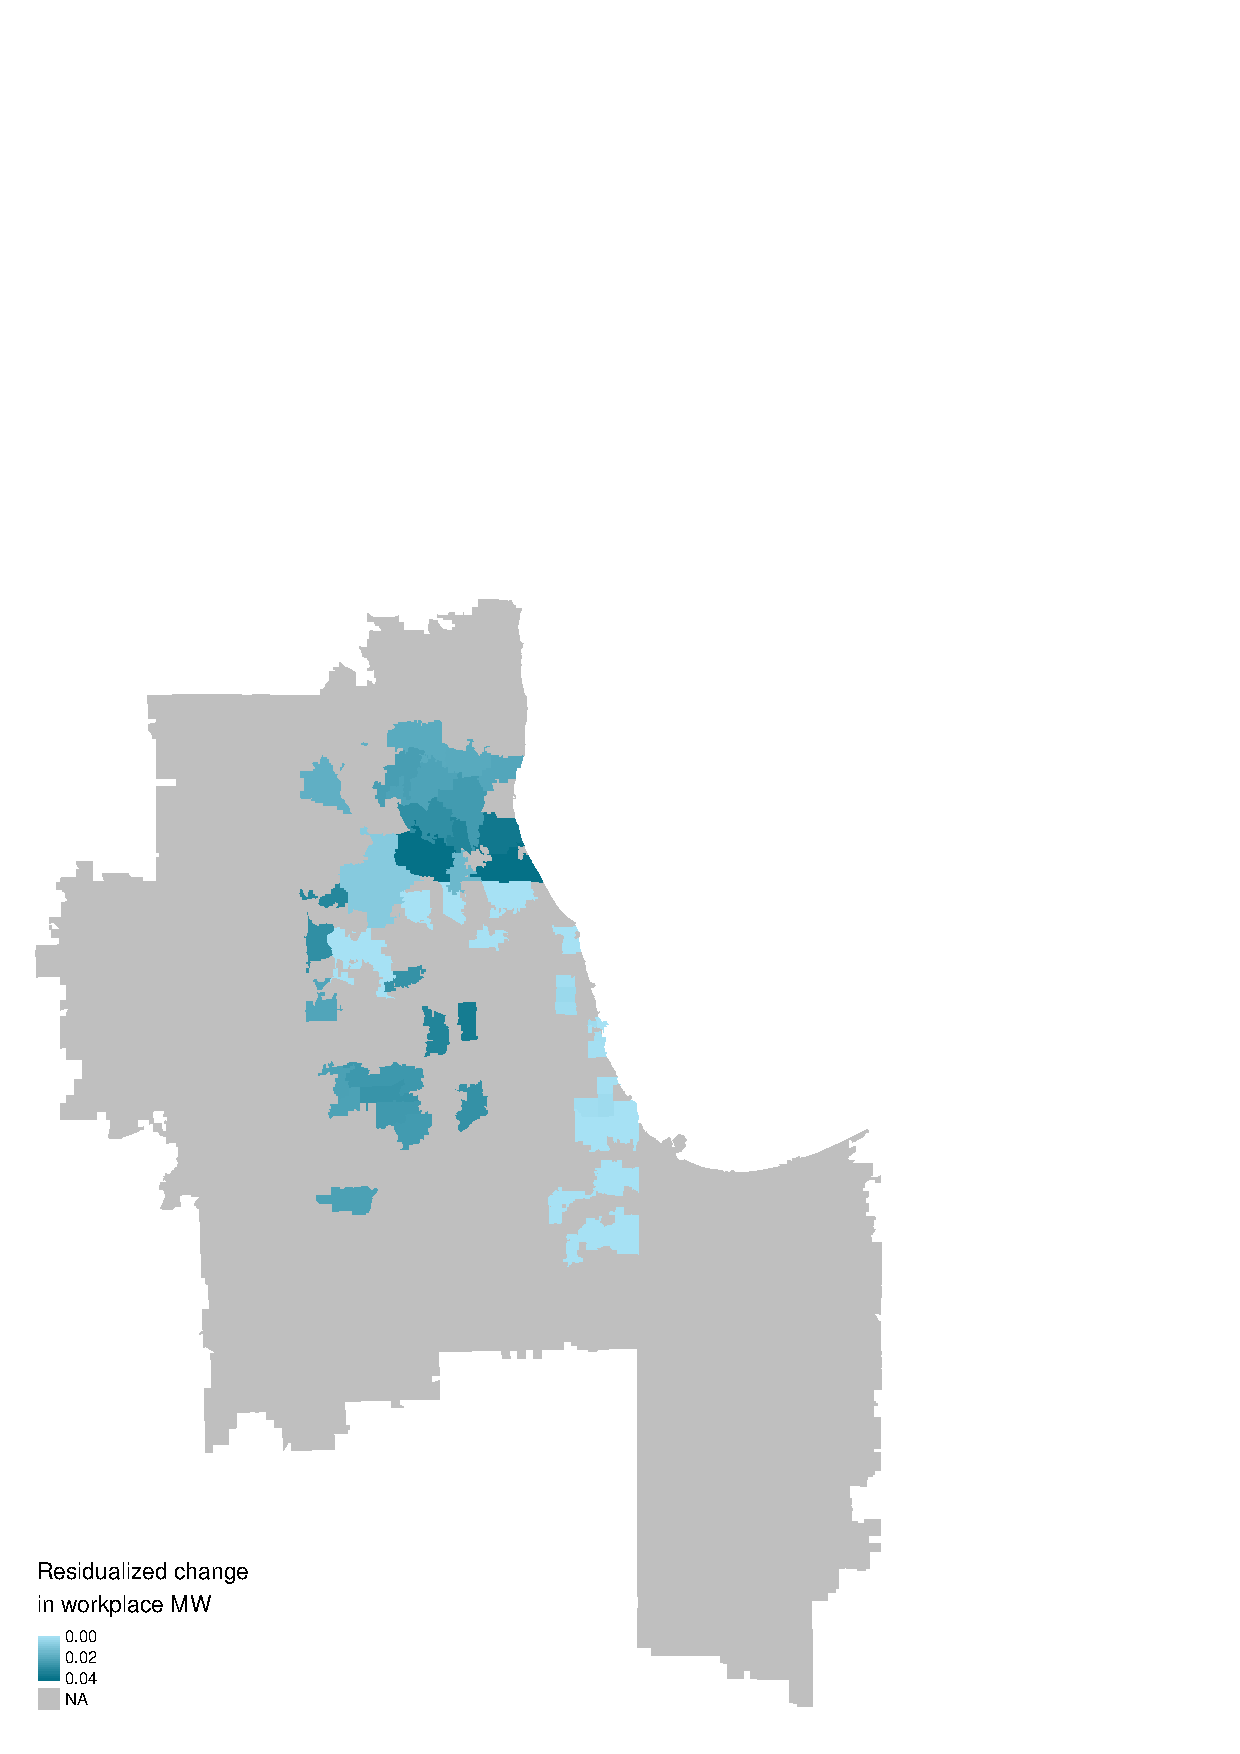
\includegraphics[width = 1\textwidth]
            {maps_events/output/chicago2019-6_r_wkp}
    \end{subfigure}%
    \begin{subfigure}{0.5\textwidth}
        \centering
        \caption*{Residualized change in log rents}
        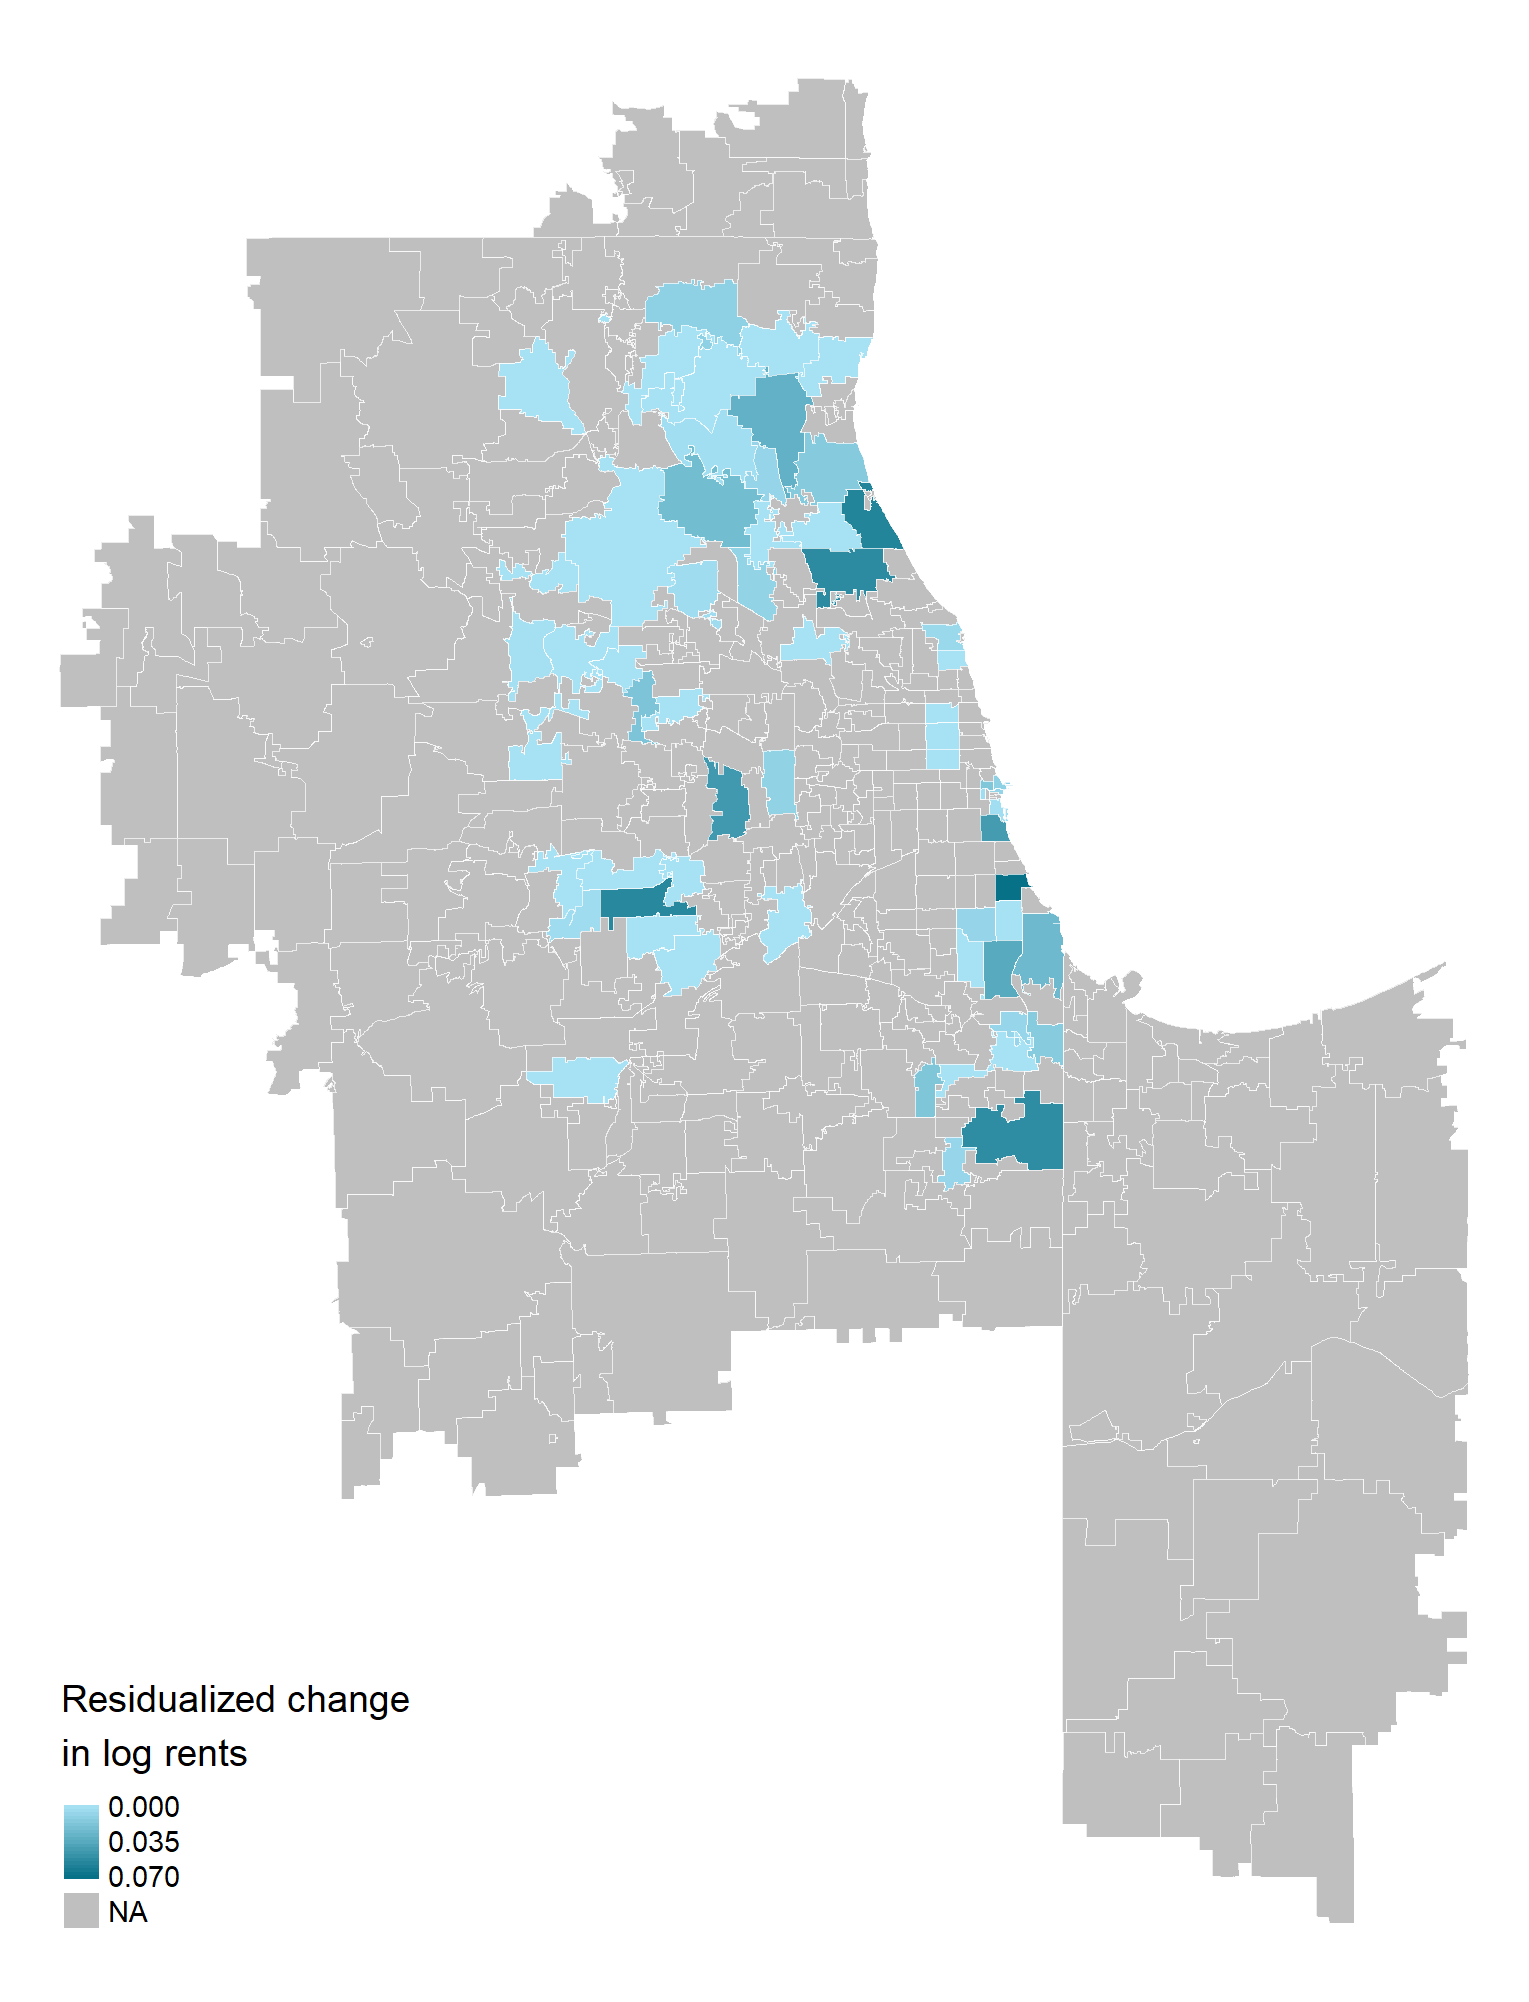
\includegraphics[width = 1\textwidth]
            {maps_events/output/chicago2019-6_r_rents}
    \end{subfigure}

    \begin{minipage}{.95\textwidth} \footnotesize
        \vspace{3mm}
        Notes: 
        Data are from the unbalanced estimation panel described in Section
        \ref{sec:data_final_panel}.
        The left figure maps the residuals of a regression of the change in the 
        workplace MW measure on the change in the residence MW measure, 
        including economic controls and year-month fixed effects.
        The right figure maps the residuals of a regression of the change in log 
        rents on economic controls and year-month fixed effects.
        The residence MW is defined as the log statutory MW in the same ZIP code.
        The workplace MW is defined as the statutory MW where the average 
        resident of the ZIP code works, constructed using LODES 
        origin-destination data.
        Economic controls from the QCEW include the change of the following 
        variables: the log of the average wage, the log of employment, and the 
        log of the establishment count for the sectors ``Information,''
        ``Financial activities,'' and ``Professional and business services.''
    \end{minipage}
\end{figure}
